% AY2017 力学 解答例
% 体裁・粒度は 参考/ のPDFに揃える（行間を埋め、最終解答は \ans{} で boxed）。
% 解答・数値・問題は本年度過去問から自力で導いた（東大版は体裁の手本のみ）。
\documentclass[11pt,a4paper]{article}
\usepackage{../../../00_common/preamble}

\usetikzlibrary{decorations.pathmorphing}

\title{力学 AY2017 解答例（専門基礎科目）}
\author{}
\date{}

\begin{document}
\maketitle

% ==================================================================
\section*{第1問〔I〕}

なめらかな床の上で，質量 $m$ の物体がばね定数 $k$ のばねにつながれて単振動する。
時刻 $t$ での変位と速度は
\[
  x=A\sin(\omega t+\alpha),\qquad v=A\omega\cos(\omega t+\alpha),
  \qquad \omega^2=\frac{k}{m}
\]
で与えられ，自然長のときの重心位置を $x=0$ とする。

\subsection*{(1) 全力学的エネルギー $E$}
床はなめらかで摩擦による散逸はなく，物体には運動エネルギーとばねの弾性
ポテンシャルエネルギーのみが寄与する。運動エネルギーは $\tfrac12 mv^2$，
自然長 $x=0$ を基準としたばねの弾性ポテンシャルエネルギーは $\tfrac12 kx^2$
であるから，全力学的エネルギーは
\[
  E=\frac12 mv^2+\frac12 kx^2 .
\]
\[
  \ans{\;E=\dfrac12 mv^2+\dfrac12 kx^2\;}
\]

\subsection*{(2) 振幅 $A$（$E$ と $k$ で表す）}
$E$ は時間によらず一定なので，任意の時刻で評価できる。変位が最大
$x=A$（端点）となる瞬間には速度が $0$（$v=0$）となるから，(1) に代入して
\begin{align*}
  E=\frac12 m\cdot 0^2+\frac12 kA^2=\frac12 kA^2
  \quad\therefore\quad A^2=\frac{2E}{k}.
\end{align*}
$A>0$ より
\[
  \ans{\;A=\sqrt{\dfrac{2E}{k}}\;}
\]

\subsection*{(3) 運動量 $p$--変位 $x$ 平面での運動の概形}
運動量は $p=mv$ である。(1) のエネルギー保存式に $v=p/m$ を代入すると
\begin{align*}
  E=\frac12 m\!\left(\frac{p}{m}\right)^{\!2}+\frac12 kx^2
   =\frac{p^2}{2m}+\frac{kx^2}{2}.
\end{align*}
両辺を $E$ で割って整理すると
\[
  \frac{x^2}{(2E/k)}+\frac{p^2}{(2mE)}=1,
\]
すなわち $(x,p)$ 平面上では原点を中心とする楕円を描く。横軸（$x$ 軸）切片は
$p=0$ より $x=\pm\sqrt{2E/k}\,(=\pm A)$，縦軸（$p$ 軸）切片は $x=0$ より
$p=\pm\sqrt{2mE}$ である。
\[
  \ans{\;\dfrac{x^2}{2E/k}+\dfrac{p^2}{2mE}=1\quad(\text{楕円}),\quad
  x\text{切片}=\pm\sqrt{\dfrac{2E}{k}},\ \ p\text{切片}=\pm\sqrt{2mE}\;}
\]

\begin{center}
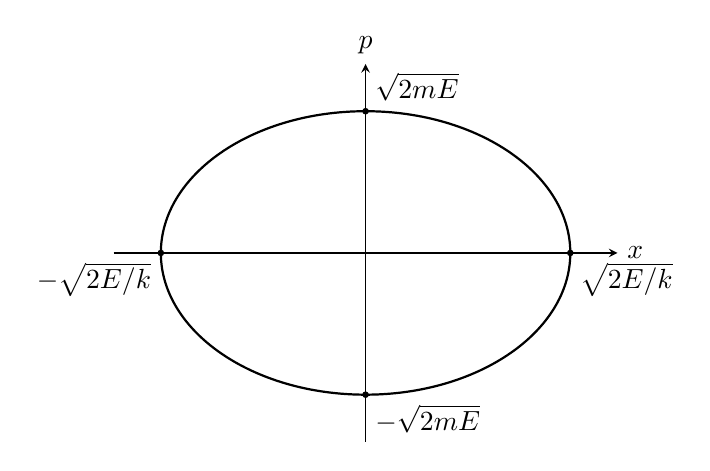
\begin{tikzpicture}[>=stealth, scale=1.0]
  \draw[->] (-3.2,0) -- (3.2,0) node[right] {$x$};
  \draw[->] (0,-2.4) -- (0,2.4) node[above] {$p$};
  \draw[thick] (0,0) ellipse (2.6 and 1.8);
  \fill (2.6,0) circle (1.2pt); \node[below right] at (2.6,0) {$\sqrt{2E/k}$};
  \fill (-2.6,0) circle (1.2pt); \node[below left] at (-2.6,0) {$-\sqrt{2E/k}$};
  \fill (0,1.8) circle (1.2pt); \node[above right] at (0,1.8) {$\sqrt{2mE}$};
  \fill (0,-1.8) circle (1.2pt); \node[below right] at (0,-1.8) {$-\sqrt{2mE}$};
\end{tikzpicture}
\end{center}

\medskip
検算: 楕円の半長・半短軸から $x_{\max}=A=\sqrt{2E/k}$，$p_{\max}=\sqrt{2mE}$。
$p_{\max}=m v_{\max}=mA\omega=m\sqrt{2E/k}\cdot\sqrt{k/m}=\sqrt{2mE}$ で
(2) の $A$ および $\omega^2=k/m$ と整合する。また端点で $E=\frac12 kA^2$，
$x=0$ で $E=\frac{p_{\max}^2}{2m}=\frac{2mE}{2m}=E$ と一致。✓

% ==================================================================
\clearpage
\section*{第2問〔II〕}

質量 $M$，長さ $L$ の一様（一定線密度）な剛体棒を，一端から $a\,(<L/2)$ の点 O を
回転中心として $xy$ 平面内で振り子運動させる。棒と $x$ 軸（鉛直下向き）のなす角を
$\theta$，重力加速度の大きさを $g$ とする。線密度は $\lambda=M/L$ である。

\subsection*{(1) 点 O まわりの慣性モーメント}
まず重心（棒の中点，一端から $L/2$）まわりの慣性モーメントを求める。重心を原点に
とり棒に沿う座標を $\xi\,(-L/2\le\xi\le L/2)$ とすると
\begin{align*}
  I_{\mathrm{G}}=\int_{-L/2}^{L/2}\xi^2\,\lambda\,d\xi
   =\lambda\left[\frac{\xi^3}{3}\right]_{-L/2}^{L/2}
   =\frac{\lambda}{3}\cdot\frac{2L^3}{8}
   =\frac{\lambda L^3}{12}=\frac{1}{12}ML^2 .
\end{align*}
点 O は一端から $a$ にあり，重心は一端から $L/2$ にあるから，O と重心の距離は
$d=\dfrac{L}{2}-a$。平行軸の定理より
\[
  I_{\mathrm O}=I_{\mathrm G}+M d^2
   =\frac{1}{12}ML^2+M\!\left(\frac{L}{2}-a\right)^{\!2}.
\]
\[
  \ans{\;I_{\mathrm O}=\dfrac{1}{12}ML^2+M\!\left(\dfrac{L}{2}-a\right)^{\!2}\;}
\]

\subsection*{(2) 点 O まわりの力のモーメントの大きさ}
重力 $Mg$ は重心に鉛直下向き（$+x$ 方向）に作用する。重心は O から距離
$d=\dfrac{L}{2}-a$ の位置にあり，棒は鉛直（$x$ 軸）から角 $\theta$ だけ傾いている。
重力線（鉛直）と回転中心 O の間の腕の長さ（重心の水平方向のずれ）は
$d\sin\theta$ であるから，力のモーメントの大きさは
\[
  N=Mg\,d\sin\theta=Mg\!\left(\frac{L}{2}-a\right)\sin\theta .
\]
\[
  \ans{\;N=Mg\!\left(\dfrac{L}{2}-a\right)\sin\theta\;}
\]

\subsection*{(3) 点 O まわりの振り子の運動方程式}
このモーメントは棒を鉛直下向き（$\theta=0$）へ引き戻す向きにはたらく復元モーメント
である。回転の運動方程式 $I_{\mathrm O}\ddot{\theta}=-N$（$\theta$ を増す向きと逆符号）
より
\[
  I_{\mathrm O}\ddot{\theta}=-Mg\!\left(\frac{L}{2}-a\right)\sin\theta,
\]
すなわち $I_{\mathrm O}=\dfrac{1}{12}ML^2+M\!\left(\dfrac{L}{2}-a\right)^{2}$ を用いて
\[
  \ans{\;\left[\dfrac{1}{12}ML^2+M\!\left(\dfrac{L}{2}-a\right)^{2}\right]\ddot{\theta}
   =-Mg\!\left(\dfrac{L}{2}-a\right)\sin\theta\;}
\]

\medskip
検算: 微小振動 $\sin\theta\simeq\theta$ では
$\ddot{\theta}=-\omega^2\theta$，$\omega^2=\dfrac{Mg(L/2-a)}{I_{\mathrm O}}
=\dfrac{g(L/2-a)}{\frac{1}{12}L^2+(L/2-a)^2}$ となり，
$a\to L/2$（O が重心）で $\omega\to0$（復元モーメントが消え振り子にならない），
$a=0$（O が一端）で $I_{\mathrm O}=\frac13ML^2$，
$\omega^2=\frac{g(L/2)}{L^2/3}=\frac{3g}{2L}$ と一様棒の物理振り子の既知結果に
一致し，次元も $[\omega^2]=\mathrm{s^{-2}}$ で妥当。✓

\end{document}
